\documentclass[a4paper,11pt]{article}
\pdfoutput=1 % if your are submitting a pdflatex (i.e.~if you have
% images in pdf, png or jpg format)

\usepackage{jheppub,amsthm} % for details on the use of the package, please
% see the JHEP-author-manual

\usepackage[utf8]{inputenc}

\usepackage{booktabs,multirow, quotes}

\usepackage[english]{babel}
\usepackage{amsmath,amssymb,graphicx,xcolor,alltt}
\usepackage{framed}

%%%%%%%%%% Start TeXmacs macros
%\catcode`\<=\active \def<{
%\fontencoding{T1}\selectfont\symbol{60}\fontencoding{\encodingdefault}}
\newcommand{\longminus}{{-\!\!-}}
\newcommand{\tmop}[1]{\ensuremath{\operatorname{#1}}}


\newcommand{\beq}{\begin{equation}}
\newcommand{\eeq}{\end{equation}}
\newcommand{\bea}{\begin{eqnarray}}
\newcommand{\ea}{\end{eqnarray}}


\theoremstyle{remark}
\newtheorem{remark}{Remark}[section]
\newtheorem{example}{Example}[section]
\theoremstyle{theorem}
\newtheorem{lemma}{Lemma}[section]

%%%%%%%%%% End TeXmacs macros
\def\red{\color{red}}

\newcommand{\SR}[1]{{\red \bf [{SR:} #1]}}
\newcommand{\junchen}[1]{\textcolor{blue}{\textbf{[JR: #1]}}}
\def\cO{\mathcal{O}}

\makeatletter
\def\@fpheader{\ }
\makeatother

\title{numerical results}

 
\author{Junchen Rong$^1$,}
\author{Slava Rychkov$^2$}

% The "\note" macro will give a warning: "Ignoring empty anchor..."
% you can safely ignore it.

\affiliation{$^1$CPHT, CNRS, \'Ecole Polytechnique, Institut Polytechnique de Paris, Palaiseau, France\\
$^2$Institut des Hautes \'Etudes Scientifiques, 91440 Bures-sur-Yvette, France}


% e-mail addresses: one for each author, in the same order as the authors
\emailAdd{junchen.rong@polytechnique.edu}
\emailAdd{slava@ihes.fr}




\abstract{aaa}%This is a note on the measurement of 3pt function using Rydberg atom experiments.}



\begin{document} 
	
	\maketitle
	
	\flushbottom


\flushbottom


\section{Periodic boundary condition}
Consider a chain of $L$ Rydberg atoms equally spaced along a circle:
\beq
	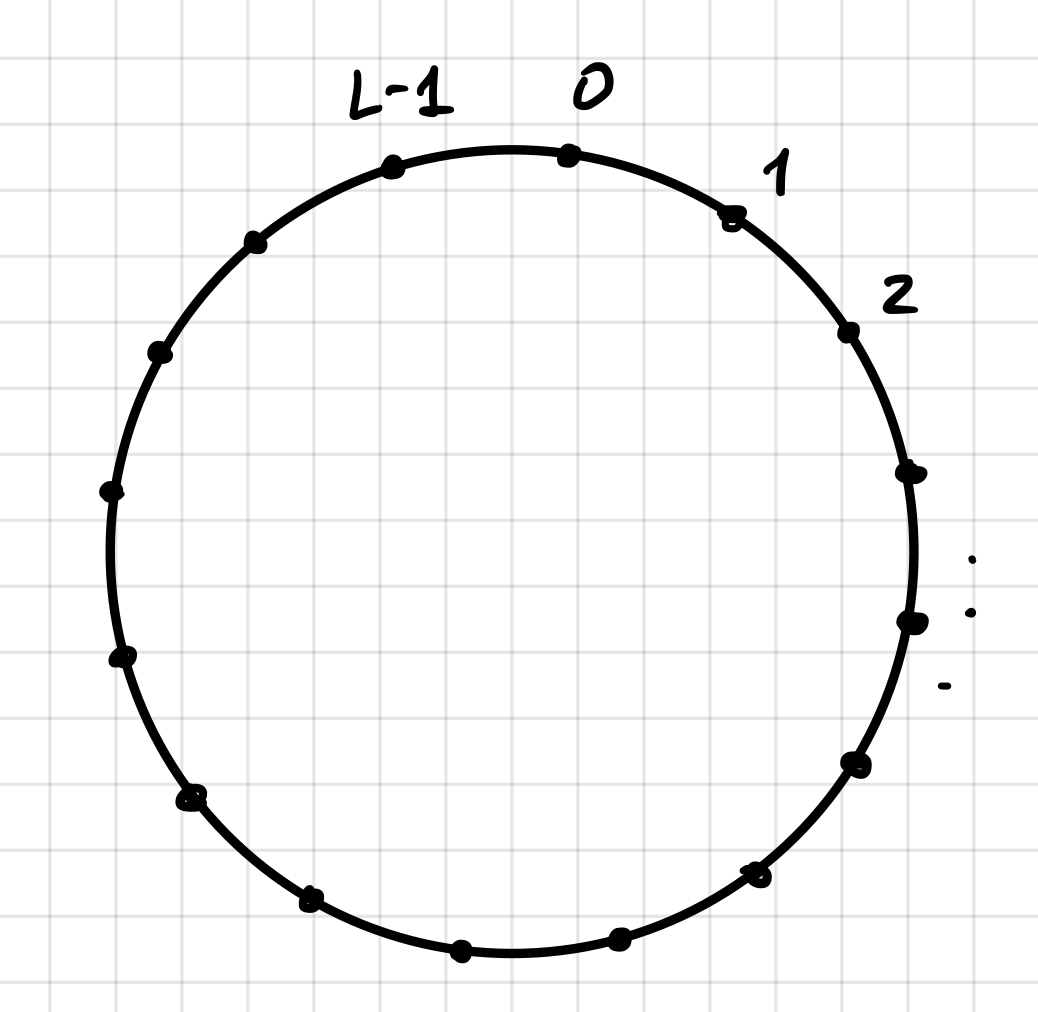
\includegraphics[width=100pt]{fig-circle.jpeg}
	\label{fig:circle}
\eeq
We describe the states in the 0-1 basis, where $|0\rangle$ ($|1\rangle$) on site $i$ corresponds to the $i$-th atom to be in the ground/Rydberg excited state.
The creation operator $a_i^\dagger$ maps $|0_i\rangle$ to $|1_i\rangle$. We have the occupation number of site $i$.
We refer to $|0\rangle$ as empty and $|1\rangle$ as occupied site. 

Using the same conventions as in~\cite{FangFang:2024eaw},  we write a realistic Hamiltonian where the atoms in the excited states interact with a repulsive $1/r^6$ interactions:
\begin{equation}
    \hat H_{phys}=\frac{\hbar \Omega}{2} \sum_i (a_i^{\dagger}+a_i) - \hbar \Delta \sum_i n_i + U \sum_{i<j}\frac{1}{d_{ij}^6}  n_{i}n_{j},\quad U=\frac{C_6}{a^6}.
    \label{eq:model}
\end{equation}
Here $a$ is distance between neighboring atoms, and $d_{ij}$ is the dimensionless distance between the $i$-th and $j$-th sites in the units of $a$
 \beq   d_{ij}=\frac{\sin(\frac{|i-j|}{L}\pi)}{\sin(\frac{1}{L}\pi)},
\eeq
(i.e. $d_{i,i+1}=1$, $d_{i,i+2}\approx 2$, etc.)

Factoring out $U$, we define the dimensionless Hamiltonian $\hat H$, as follows:
\begin{align}
	\hat H_{phys}&= U\hat H\\
	\hat H &= \frac{\Omega'}{2} \sum_i (a_i^{\dagger}+a_i) - \Delta' \sum_i n_i + \sum_{i<j}\frac{1}{d_{ij}^6}  n_{i}n_{j}
	\label{eq:modelp}\\
	\Omega' &= \hbar \Omega/U,\quad
	\Delta' = \hbar \Delta/U\,.
\end{align}
$\Omega'$ and $\Delta'$ are real dimensionless numbers. The sign of $\Omega'$ is unimportant as it can flipped by redefining $|1\rangle \to -|1\rangle$.
%\begin{align}
%d^{\dagger}|0\rangle \rightarrow -d^{\dagger}|0\rangle. 
%\end{align}
The experimentally accessible parameter space is, roughly, \cite[Tab. 1]{noise-note}
\begin{align}
\Omega' \in [0,2],\quad \Delta' \in[-10,20].
\end{align}
The phase diagram near the Ising transition is reported in Fig.~\ref{phasediagramHBlong}.
\begin{figure}[htbp]
\centering
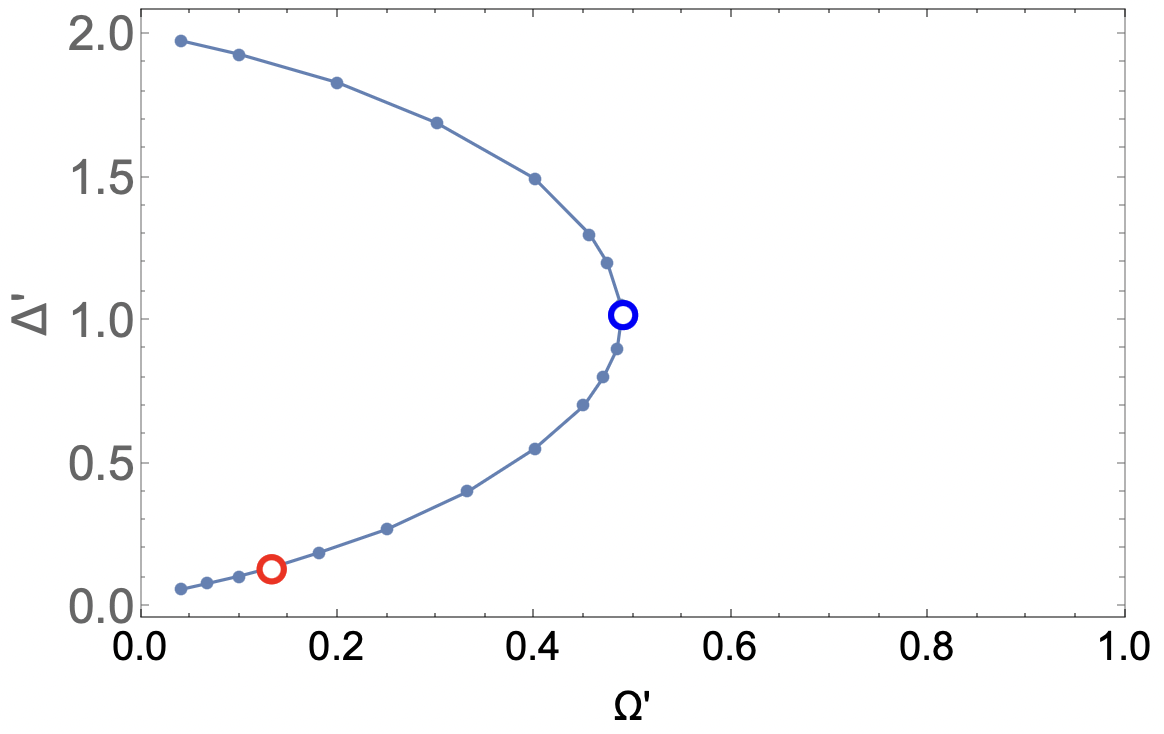
\includegraphics[width=0.6\textwidth]{phase_diagram_SSF_LR.png}
\caption{The phase diagram of the Rydberg model \eqref{eq:model}. The red circle corresponds to the point studied in~\cite{FangFang:2024eaw}. The red circle corresponds to the point with exact $\mathbb{Z}_2$ symmetry.} 
\label{phasediagramHBlong}
\end{figure}

We can pass from the $0,1$ basis to $\pm 1$ basis. In this basis we have $n_i=(1+\sigma^z_i)/2$, $a_i+a^\dagger_i=\sigma^x_i$. The Hamiltonian becomes
\beq
\hat H = \frac{\Omega'}{2} \sum_i \sigma^x_i + \sum_{i<j}\frac{1}{4d_{ij}^6}  \sigma^z_{i}\sigma^z_{j}+ \frac 12 (\sum_{j=1}^{L-1} \frac{1}{2d_{j0}^6} - \Delta') \sum_{i}  \sigma^z_{i} + const
\eeq
We have
\beq
\sum_{j=1}^{L-1} \frac{1}{2d_{j0}^6} = \zeta(6) +O(1/L^2)=1.01734\ldots+O(1/L^2)
\eeq
For $\Delta'=\zeta(6)$ the model has the exact $\mathbb{Z}_2$ symmetry. This is the "tip of the parabola" in Fig. \ref{phasediagramHBlong}. On the line $\Delta'=\zeta(6)$ the model is very nearly approximated by the transverse field Ising model (TFIM). The phase transition in the TFIM would be at $\Omega'=1/2$. The phase diagram is symmetric with respect to $\Delta'=\zeta(6)$.

For general $\Delta'\in(0,1)$, the Hamiltonian $\hat H$ does not have onsite $\mathbb{Z}_2$ symmetry. But the phase transition is still in the $\mathbb{Z}_2$-symmetric Ising-CFT universality class. The $\mathbb{Z}_2$ symmetry of the CFT will emerge from a lattice translation by one lattice unit. (In the broken phase, the expectation value $\langle n_i \rangle$ is periodic with period 2, and shift by one lattice unit permutes the two ground states.) This will have to be taken into account when constructing lattice operators which represent CFT operators.

The region $\Omega'\ll 1$ and $\Delta'\ll 1$ corresponds to strong Rydberg blockade, which can be effectively described by the Fendley-Sengupta-Sachdev model. 

We now measure the two point function $\langle \sigma\sigma\rangle$. At r $\Delta'=\zeta(6)$, we have the map
$$\sigma(x)\sim b~(-1)^x Z_x.$$
The non-universal constant $b$ is model dependent. We take $L=40$, at $\Delta'=\zeta(6)$, the critical point is located at $\Omega'=0.488$. The two point function is shown in Fig.~\ref{ZZ2pt}. We have used the definition
$$
|x|_L:= \frac{L}{\pi} \sin\left(\frac{\pi}{L} |x|\right)
$$
\begin{figure}[htbp]
\centering
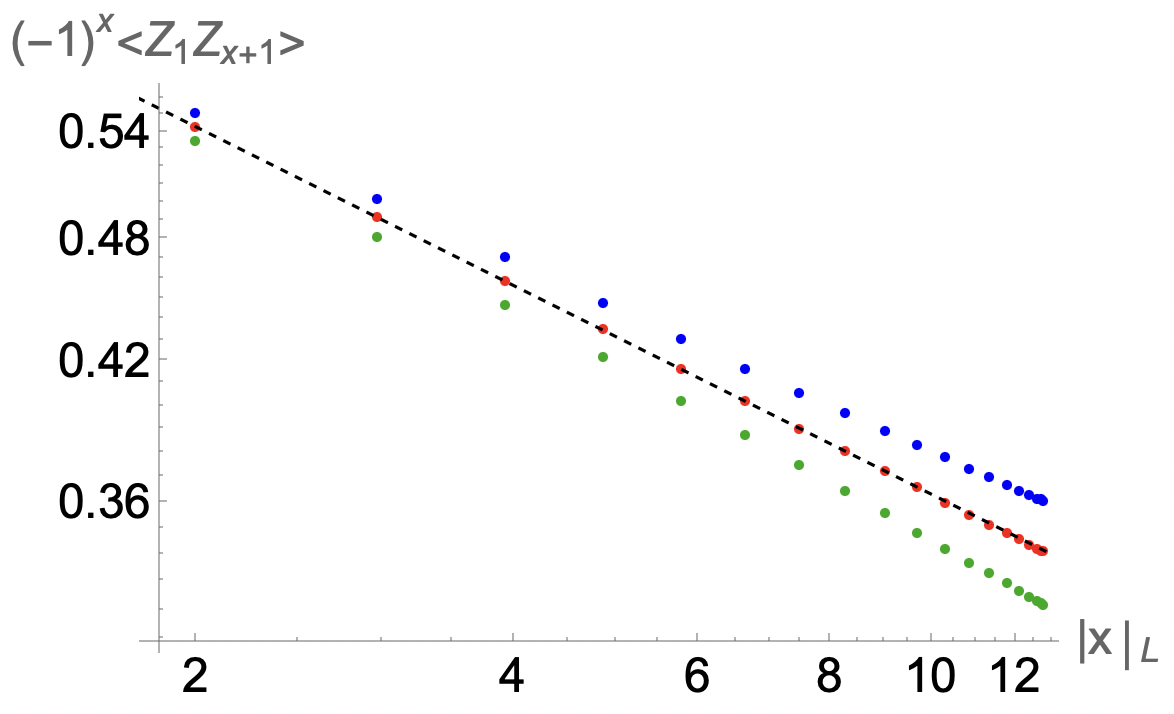
\includegraphics[width=0.6\textwidth]{ZZ_correlation.png}
\caption{The correlation function $(-1)^x \langle Z_i Z_{x+i}\rangle$. The red, green, blue curves correspond to $\Omega'=0.488,~0.490,$ and $0.486$ respectively. The black dashed line is $\frac{0.645}{|x_L|^{1/4}}$.} 
\label{ZZ2pt}
\end{figure}

\section{Open boundary condition}
In the case of open boundary condition,
\beq
\hat H = \frac{\Omega'}{2} \sum_i \sigma^x_i + \sum_{i<j}\frac{1}{4d_{ij}^6}  \sigma^z_{i}\sigma^z_{j}+ \frac 12 \sum_{i}  \left(\sum_{j\neq i}^{L}( \frac{1}{2d_{ji}^6} - \Delta'_i) \sigma^z_{i} \right)+ const
\eeq
We take take $\Delta'_i=1.01734$ and $\Omega=0.488$, then the bulk is in the critical phase. At the boundary, this breaks the $\mathbb{Z}_2$ symmetry, and prefers $\langle Z_i\rangle<0$. To avoid that, we take 
\beq\label{boundarytuning}
\Delta'_1=\Delta'_N=-5.
\eeq
I believe a spatial dependent $\Delta'$ is not hard, as discussed in \cite{Sun:2026aqf}, see the section ``Boundary tuning of TCI CFT''. 
Notice that we have to put odd number of atoms, due to the anti-ferromagnetic nature of model, we take $N=41$. The one-point function we got is shown in Fig.~\ref{Z1pt}.
\begin{figure}[htbp]
\centering
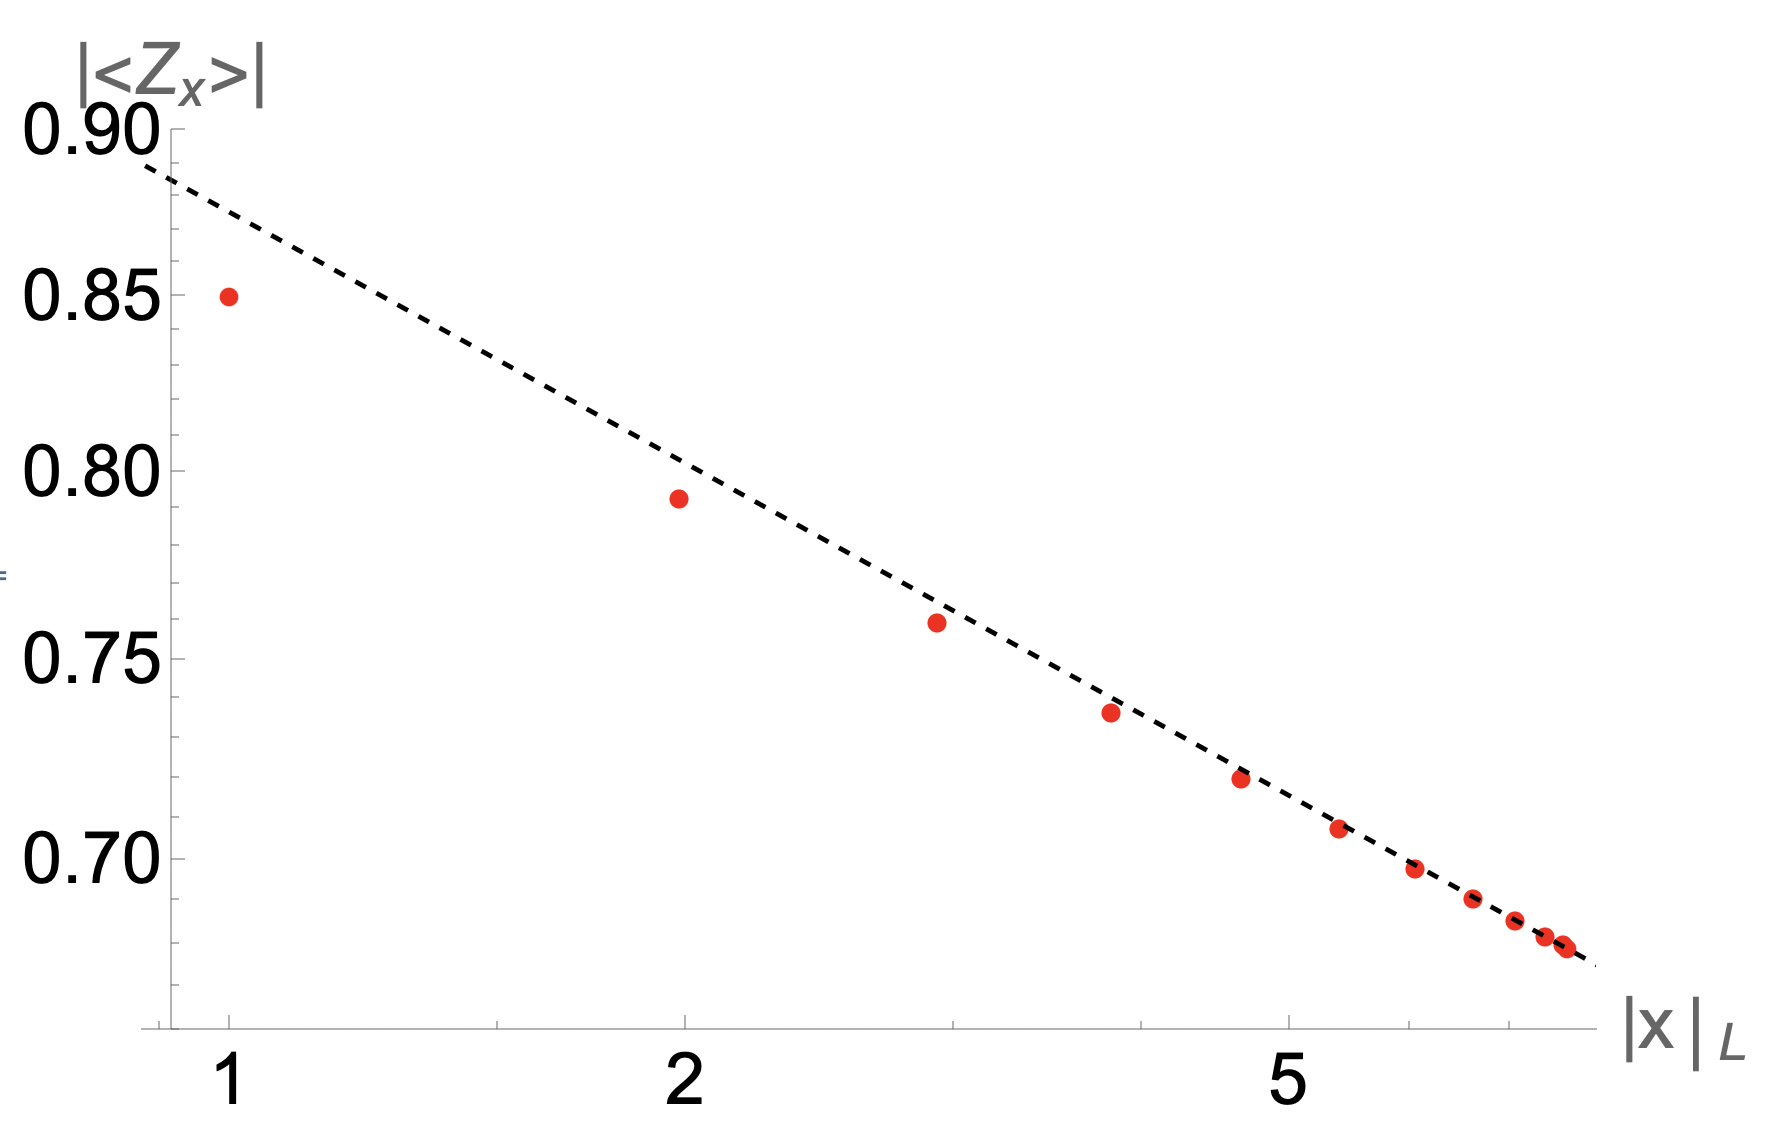
\includegraphics[width=0.6\textwidth]{Z1pt.png}
\caption{The correlation function $|\langle Z_x \rangle|$. The red and blue dots corresponds to $\Delta'_1=\Delta'_N=1.01734$ (uniform $\Delta'$) and $\Delta'_1=\Delta'_N=5$ respectively. The black dashed line is $\frac{0.88}{|x_L|^{1/8}}$.} 
\label{Z1pt}
\end{figure}

If we instead take $N$ to be even, for example $N=40$, this means that we are taking spin-up boundary condition on one end and the spin-down boundary condition on the other end. Performing a conformal map to upper half plane, this means we have put a pair of boundary changing operators, one at the origin and the other at infinity. The 3rd operator $\sigma$ operator is at the unit semi-circle. \junchen{work out this explicitly.}

\bibliography{reference.bib}
\bibliographystyle{utphys}

\end{document}
